\section{Implementation}
\label{sec:imp}
The algorithm presented so far is idealized and unoptimized.
In this section, we discuss refinements that improve the 
quality of the inferred descriptions and/or improve performance.

\subsection{Token families}
So far, parsing a \cd{Sync} token yields
one of three results: \cd{Good}, \cd{Fail} or \cd{Recovered}. 
In the actual implementation, a \cd{Sync} token can be not only a constant string, but also
a constant integer, an integer range or a combination thereof.
Consider parsing the token \cd{Sync (Str "GET")} when
the current input starts with ``POST.'' The
\cd{parse\_base} function indicates the result should be \cd{Fail}.
In reality, the input ``POST'' is in the same {\em family} as ``GET,'' 
\ie{}, a word,
and it may very well be that this \cd{Sync} token should have been 
an enumeration of words rather than a single word.
To handle such cases, we created a fourth type of parse node, \cd{Partial}, 
to indicate that the input belongs to the same family as the expected
token but does not match exactly, \ie, it is {\em partially} correct.
During aggregation, partial nodes cause the description 
to be specialized to include the additional values.  In the above example, the aggregate 
function will change the description to \cd{Sync (Enum [Word "GET", Word "POST"])}.
Such partial nodes reduce the number of parsing errors
and produce more compact and meaningful descriptions.


\subsection{Rewriting rules}
When the incremental learning algorithm produces a refined description
from an aggregate, the algorithm applies rewriting rules
to the new description to improve its quality and readability.
Most of the rules are data-independent and inherited from \learnpads{}, such as 
removing degenerate lists and flattening nested structs and unions.
We introduce one new {\em data dependent} rule called {\em MergeOpts}
to optimize a type pattern that occurs frequently during incremental
learning.  Recall that the aggregate function
introduces \cd{Opt} nodes above a \cd{BaseA} or \cd{SyncA} node 
whenever the corresponding \cd{Base} or \cd{Sync} token in the description failed to 
parse. When faced with an entirely new form of data, 
the algorithm is likely to introduce a series of \cd{Opt} nodes as
each type in the original description fails in succession. 
The {\em MergeOpts} rule collapses these consecutive \cd{Opt} nodes if they
are correlated, \ie{}, either they are all always present or all always
absent.  To verify this correlation, the algorithm maintains a
table that records the branching decisions when parsing each
data line. It uses this table to determine whether to merge
adjacent \cd{Opt} nodes during rewriting. 
\figref{fig:opts} illustrates the effect of this rule.  In the figure,
$S$ denotes a struct and $B$ a base token.

\begin{figure}[t]
\begin{center}
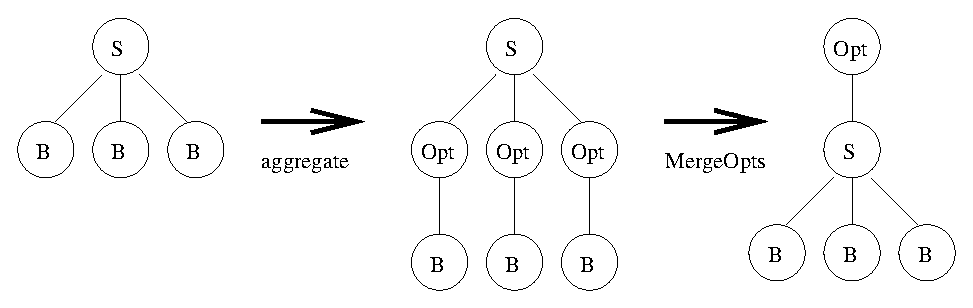
\epsfig{file=opts.eps,width=\columnwidth}
\caption{MergeOpts rewriting rule}\label{fig:opts}
\vskip -2ex
\end{center}
\end{figure}


\subsection{Performance}
The pseudo-code in \figref{fig:inc-learning} suggests the number of
aggregates is of the order $O(m ^ n)$, where $m$ is the maximum number of
parses for a line of input  and $n$ is the number of lines to
aggregate.  Clearly, this algorithm will not scale 
unless $m$ and $n$ are bounded.

We have implemented several optimizations to limit the number of 
parses and aggregates. First, we do not return all possible
parses when parsing a description component \cd{D}. 
Instead, we rank the parses by a metric that
measures their quality and return only the top $k$. The metric is
a triple: 
$m = (e,~ s,~ c)$,
where $e$ is the number of errors, $s$ is the number of 
characters skipped during \cd{Sync} token recovery, and $c$ is the number
of characters correctly parsed. The metric is considered \textit{perfect} if $e = 0$.
Metric $m_1$ is better than $m_2$ if $m_1$ is perfect and $m_2$ is not, or
if 
\[\frac{c_1}{s_1+c_1} > \frac{c_2}{s_2 + c_2}.\]

In practice, \cd{parse} returns a list of
{\em parse triples} $(r,~m,~j)$, where $r$ is the data representation of
the parse, $m$ is the metric associated with $r$, and
$j$ is the position in the input after the parse.
We define a \cd{clean} function that first partitions the
triples into groups that share the same 
{\em span}, \ie{}, the substring of the input consumed by the parse.
For each group, \cd{clean} retains all perfect parses. If 
none exists, it retains the best parse in the group. 
We justify discarding the other triples because
given a description $d$ and a fixed span, we always
prefer the parse with the best metric. This idea is
similar to the dynamic programming techniques used in 
Earley Parsers \cite{earley-parser}. Finally \cd{clean} returns all
the perfect triples plus up to the top $k$ non-perfect triples.
The \cd{clean} function reduces the number of bad parses 
to a constant $k$ while guaranteeing that if there is a
perfect parse, it will be returned. 

A second optimization, which we call {\em parse cut-off}, terminates a
candidate parse when parsing a struct with multiple
fields $f_1$, $f_2$, ..., $f_n$ if the algorithm encounters 
a threshold number of errors in succession. 
This technique may result in no possible parses for the
top-level description.  In this case, we restart the process
with the parse cut-off optimization turned off. 
A third optimization is memoization.
The program keeps a global memo table indexed by the pair of a
description \cd{D} and the beginning position for parsing \cd{D} which
stores the result for parsing \cd{D} at the specific position.
Finally, we bound the total number of aggregates the
algorithm can produce by selecting the top
$k$ aggregates with the fewest number of \cd{Opt} and \cd{Learn}
nodes. 


